\documentclass{beamer}
\usepackage[utf8]{inputenc}

\usetheme{Madrid}
\usecolortheme{default}
\usepackage{amsmath,amssymb,amsfonts,amsthm}
\usepackage{txfonts}
\usepackage{tkz-euclide}
\usepackage{listings}
\usepackage{adjustbox}
\usepackage{array}
\usepackage{tabularx}
\usepackage{gvv}
\usepackage{lmodern}
\usepackage{circuitikz}
\usepackage{tikz}
\usepackage{graphicx}
\usepackage{multicol}
\setbeamertemplate{page number in head/foot}[totalframenumber]

\usepackage{tcolorbox}
\tcbuselibrary{minted,breakable,xparse,skins}



\definecolor{bg}{gray}{0.95}
\DeclareTCBListing{mintedbox}{O{}m!O{}}{%
  breakable=true,
  listing engine=minted,
  listing only,
  minted language=#2,
  minted style=default,
  minted options={%
    linenos,
    gobble=0,
    breaklines=true,
    breakafter=,,
    fontsize=\small,
    numbersep=8pt,
    #1},
  boxsep=0pt,
  left skip=0pt,
  right skip=0pt,
  left=25pt,
  right=0pt,
  top=3pt,
  bottom=3pt,
  arc=5pt,
  leftrule=0pt,
  rightrule=0pt,
  bottomrule=2pt,

  colback=bg,
  colframe=orange!70,
  enhanced,
  overlay={%
    \begin{tcbclipinterior}
    \fill[orange!20!white] (frame.south west) rectangle ([xshift=20pt]frame.north west);
    \end{tcbclipinterior}},
  #3,
}
\lstset{
    language=C,
    basicstyle=\ttfamily\small,
    keywordstyle=\color{blue},
    stringstyle=\color{orange},
    commentstyle=\color{green!60!black},
    numbers=left,
    numberstyle=\tiny\color{gray},
    breaklines=true,
    showstringspaces=false,
}
%------------------------------------------------------------
%This block of code defines the information to appear in the
%Title page
\title %optional
{1.2.12}
%\subtitle{A short story}

\author % (optional)
{BEERAM MADHURI - EE25BTECH11012}



\begin{document}


\frame{\titlepage}
\begin{frame}{Question}
For $|x| < 1$, $\coth(x)$ can be approximated as: \hfill (EC 2007)

\begin{enumerate}
    \item[a)] $x$
    \item[b)] $x^2$
    \item[c)] $\dfrac{1}{x}$
    \item[d)] $\dfrac{1}{x^2}$
\end{enumerate}

\end{frame}
\begin{frame}{Solution}
\textbf{Solution:}\\
The hyperbolic cotangent function is defined as:

\begin{align}
    \coth(x) = \frac{\cosh(x)}{\sinh(x)}
\end{align}

To find the approximation for small x, we use the Taylor Series expansions for $\cosh(x)$ and $\sinh(x)$ centered at 0:
Expansion of cosh(x) and sinh(x)
\begin{align}
    \cosh(x): 1 + \frac{x^2}{2!} + \frac{x^4}{4!} + \dots\\
    \sinh(x): x + \frac{x^3}{3!} + \frac{x^5}{5!} + \dots
\end{align}
\end{frame}
\begin{frame}
Now, substitute these into the $\coth(x)$ formula:
\begin{align}
    \coth(x) = \frac{1 + \frac{x^2}{2} + \dots}{x + \frac{x^3}{6} + \dots}
\end{align}
For very small values of x, we can focus on the dominant terms (the lowest power of x in the numerator and denominator):
\begin{align}
    \coth(x) \approx \frac{1}{x}
\end{align}

Correct Option: c) $\frac{1}{x}$
\end{frame}

\begin{frame}[fragile]
\frametitle{C Code}
\begin{lstlisting}
#include <stdio.h>
#include <math.h>

double calculate_coth(double x) {
    if (x == 0.0) {
        printf("Error: coth(0) is undefined.\n");
        return NAN; // Returns 'Not a Number'
    }
    // Standard formula: cosh(x) / sinh(x)
    return cosh(x) / sinh(x);
}
\end{lstlisting}
\end{frame}

\begin{frame}[fragile]
\frametitle{C Code}
\begin{lstlisting}
int main() {
    double x;

    printf("Enter the value of x: ");
    if (scanf("%lf", &x) != 1) {
        printf("Invalid input.\n");
        return 1;
    }
    double result = calculate_coth(x);

    if (!isnan(result)) {
        printf("coth(%.4f) = %.6f\n", x, result);
    }

    return 0;
}
\end{lstlisting}
\end{frame}

\begin{frame}[fragile]
\frametitle{Python Code}
\begin{lstlisting}
import numpy as np
import matplotlib.pyplot as plt

x = np.linspace(-2, 2, 400)
x = x[x != 0] 

# Define the functions
coth_x = 1 / np.tanh(x)
approx_x = 1 / x

plt.figure(figsize=(10, 6))
plt.plot(x, coth_x, label=r'$\coth(x)$', color='blue', linewidth=2)
plt.plot(x, approx_x, '--', label=r'Approximation $\frac{1}{x}$', color='red', linewidth=2)
\end{lstlisting}
\end{frame}

\begin{frame}[fragile]
\frametitle{Python Code}
\begin{lstlisting}
plt.ylim(-10, 10)
plt.axhline(0, color='black',linewidth=0.5)
plt.axvline(0, color='black',linewidth=0.5)
plt.title(r'Comparison of $\coth(x)$ and its Approximation $\frac{1}{x}$', fontsize=14)
plt.xlabel('x', fontsize=12)
plt.ylabel('f(x)', fontsize=12)
plt.legend()
plt.grid(True, linestyle='--', alpha=0.7)

# Highlight the region |x| < 1
plt.fill_between(x, -10, 10, where=(np.abs(x) < 1), color='green', alpha=0.1, label='Region $|x| < 1$')

plt.show()
\end{lstlisting}
\end{frame}

\begin{frame}{Plot}
\begin{figure}
\centering
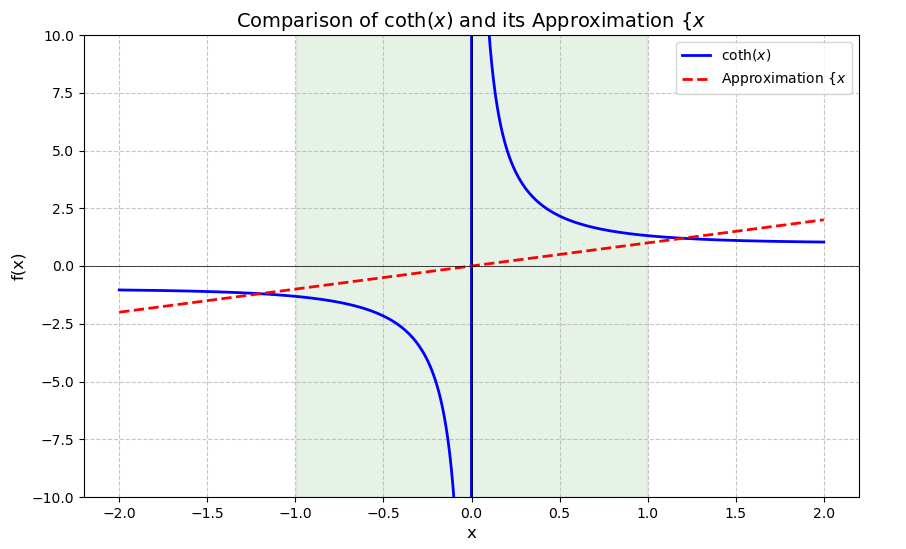
\includegraphics[width=0.75\columnwidth]{Figures/a.png}
\caption{Coth(x) and x comparision for $|x|<1$}
\label{fig:placeholder}
\end{figure}
\end{frame}

\begin{frame}
\begin{figure}
\centering
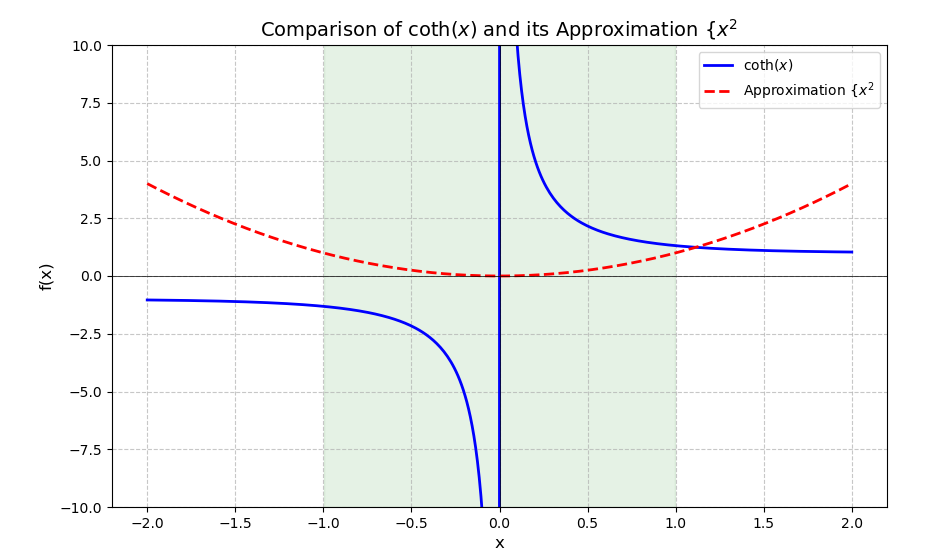
\includegraphics[width=0.75\columnwidth]{Figures/b.png}
\caption{Coth(x) and $x^2$ comparision for $|x|<1$}
\label{fig:placeholder}
\end{figure}
\end{frame}

\begin{frame}
\begin{figure}
\centering
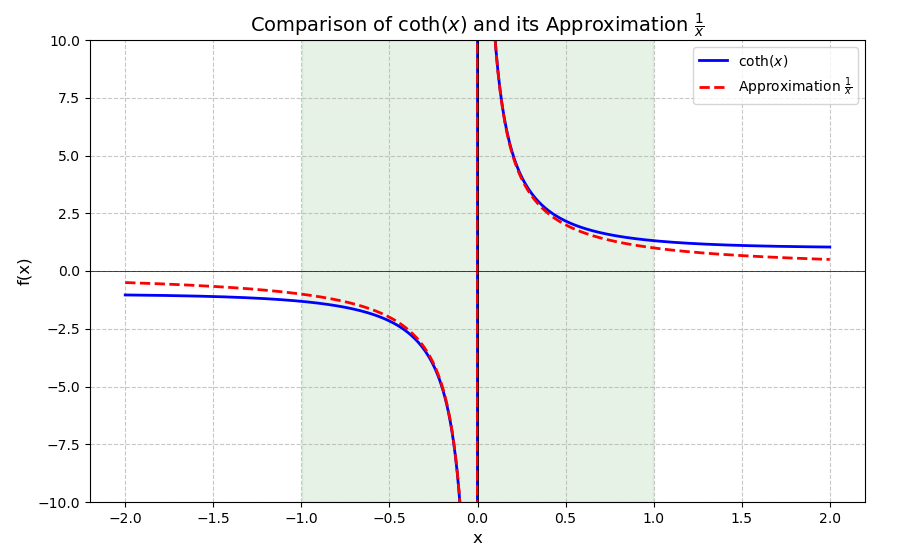
\includegraphics[width=0.75\columnwidth]{Figures/c.png}
\caption{Coth(x) and 1/x comparision for $|x|<1$}
\label{fig:placeholder}
\end{figure}
\end{frame}

\begin{frame}
\begin{figure}
\centering
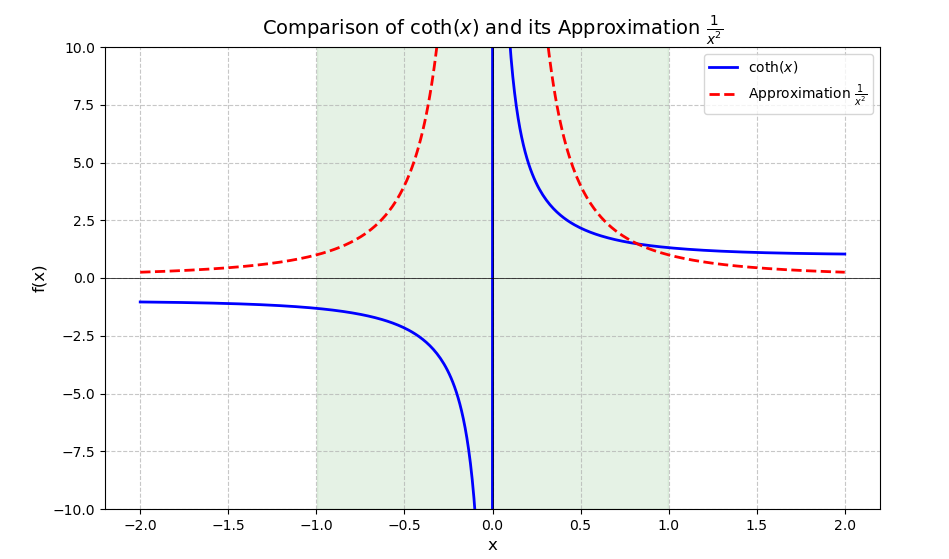
\includegraphics[width=0.75\columnwidth]{Figures/d.png}
\caption{Coth(x) and $1/x^2$ comparision for $|x|<1$}
\label{fig:placeholder}
\end{figure}
\end{frame}
\end{document}